\usepackage{pgfplots}
\pgfplotsset{compat=1.15}
\usepackage{tikz, tikz-3dplot}
\usetikzlibrary{calc}
\usetikzlibrary{patterns}
\usetikzlibrary{backgrounds}
\usetikzlibrary{decorations.pathmorphing}
\usetikzlibrary{decorations.markings}%\usetikzlibrary{tqft}
\usetikzlibrary{spath3}

% Default TikZ option: draw all paths unless overridden
\tikzset{vcenter/.style={baseline=(current bounding box.center)}}
\tikzset{every picture/.style={label distance =-2mm,>=stealth, semithick}}
%\tikzset{tqft/cobordism/.style={draw}}
%\tikzset{tqft/every boundary component/.style = {draw}}
\tikzset{dotnode/.style={fill,circle,inner sep=1pt}}
\tikzset{midarrow/.style={postaction={decorate},
                 decoration={
                    markings,% switch on markings
                    mark=at position #1 with {\arrow{>}},
                 }},
        midarrow/.default=0.5
}
\tikzset{morphism_sq/.style = {rectangle, inner sep=3pt,draw = black!50,
minimum size=18pt,scale=0.8}}
\tikzset{morphism/.style = {circle,draw,inner sep=1pt, minimum
size=18pt, scale=0.8}}
\tikzset{stringnode/.style={rectangle, inner sep=5pt, draw = black!50, fill=black!10}}
\tikzset{2morphism/.style={line width=0.6pt, double distance=1.5pt}}
\tikzset{squiggly/.style={decorate,decoration={snake,amplitude=1mm,segment length=3mm, post=lineto, post length=2mm},}}
\tikzset{blue_dot/.style={pattern color = blue, pattern = dots}}
\tikzset{red_lines/.style={pattern color = red, pattern = north west lines}}
\tikzset{lightblue/.style={fill=blue!15}}
\tikzset{lightred/.style={fill=red!40}}
\tikzset{lightyellow/.style={fill=yellow!35}}
\tikzset{euler/.style={fill,circle,inner sep=1.5pt, draw = black!50, fill=red}}
\tikzset{regular/.style={densely dashed}}
\tikzset{drinfeld center/.style ={green!60!black, double
distance=1pt}}
\tikzset{overline/.style={preaction={draw,line
width=2mm,white,-},semithick,>=stealth}}
%drinfeld center=[>=stealth,green!60!black, double
%distance=1pt]]

\tikzset{rigidity/.pic = {
    \draw [pic actions]  (0,0)--(0,-1) arc (-180:0:0.25) arc (180:0:0.25) -- +(0,-1);
  }
  }
\tikzset{coev/.pic = {
    \draw [pic actions]  (0,0) arc (180:0:0.25);
  }
}
\tikzset{ev/.pic = {
    \draw [pic actions]  (0,0) arc (-180:0:0.25);
  }
}
\tikzset{mult/.pic = {
    \node[dotnode] (o) at (0,0){};
    \draw [pic actions]  (-0.25,0.5)--(o)--(0.25,0.5);
    \draw [pic actions]  (o)--(0,-0.5);
  }
}
\tikzset{comult/.pic = {
    \node[dotnode] (o) at (0,0){};
    \draw [pic actions]  (-0.25,-0.5)--(o)--(0.25,-0.5);
    \draw [pic actions]  (o)--(0,0.5);
  }
}


%----- Tikz setup for Chapter13------------
% This environment will ensure that Tikz definitions of Chapter 13 don't 
% accidentally interfere with any other chapters.
\newenvironment{defectfiguresetup}
{
	\begingroup
		\pgfdeclarelayer{nodelayer}
		\pgfdeclarelayer{edgelayer}
		\pgfdeclarelayer{labels}
		\pgfsetlayers{edgelayer,nodelayer,labels,main}
		\tikzset{
			none/.style={},
			0cell/.style={circle, fill=green, draw=green!80!green, line width=0.4pt, inner sep=1.5pt},	
			1cell/.style={draw=green, line width=0.8pt},
			defect/.style={draw=red, line width=1.2pt},
			junction/.style={circle, fill=black, draw=black!80!black, line width=0.4pt, inner sep=1.8pt},
		}
}
{
	\endgroup
}
%-----end of Tikz setup for Chapter13------------


\usepackage{tikz-cd}




\usetikzlibrary{shapes.geometric}
\usetikzlibrary{calc}
%\newcommand{\tikzsetup}{
%  \tikzstyle tikzdefault=[semithick,>=stealth];
%  \tikzstyle dotnode=[fill,circle,inner sep=1pt];
%  \tikzstyle morphism=[circle,draw,inner sep=1pt, minimum
%size=18pt, scale=0.8];
%  \tikzstyle coupon=[draw,inner sep=1pt, minimum size=18pt,scale=0.8];
%  \tikzstyle overline=[preaction={draw,line
%width=2mm,white,-},semithick,>=stealth];
%  \tikzstyle drinfeld center=[>=stealth,green!60!black, double
%distance=1pt]];
%  \tikzstyle cell=[fill=black!10,draw, very thin];
%   \tikzstyle midarrow=[fill, dart, dart tail angle=112,
%    dart tip angle=53,inner sep=0.55pt,sloped,allow upside down];
%   \tikzstyle revmidarrow=[fill, dart, dart tail angle=112,
%    dart tip angle=53,inner sep=0.55pt,sloped,
%    allow upside down,rotate=180];
%}
%%

%%%%%%%%%%%%%%%%%%%%%%%%%%%%%%%%
%%% This tikzsetup is being used in Section 19.4 %%%%%%
%%% This was copied from \ocite{balsam-kirillov} %%%%%%
%%%  If it breaks something, we should remove it %%%%%%
\newcommand{\tikzsetup}{
	\tikzstyle tikzdefault=[semithick,>=stealth];
	\tikzstyle dotnode=[fill,circle,inner sep=1pt];
	\tikzstyle morphism=[circle,draw,inner sep=1pt, minimum
	size=18pt, scale=0.8];
	\tikzstyle coupon=[draw,inner sep=1pt, minimum size=18pt,scale=0.8];
	\tikzstyle overline=[preaction={draw,line
		width=2mm,white,-},semithick,>=stealth];
	\tikzstyle drinfeld center=[>=stealth,green!60!black, double
	distance=1pt]];
	\tikzstyle cell=[fill=black!10,draw, very thin];
	\tikzstyle midarrow=[fill, dart, dart tail angle=112,
	dart tip angle=53,inner sep=0.55pt,sloped,allow upside down];
	\tikzstyle revmidarrow=[fill, dart, dart tail angle=112,
	dart tip angle=53,inner sep=0.55pt,sloped,
	allow upside down,rotate=180];
}
%%%%%%%%%%%%%%%%%%%%%%%%%%%%%%%%

%%%%%%%%%%%%%%%%%%%%%%%%%%%
\newcommand{\tzPairingIII}{
	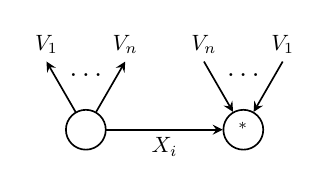
\begin{tikzpicture}[baseline=0pt]
		\tikzsetup
		\node[morphism] (ph) at (0,0) {$\ph$};
		\node[morphism] (ph*) at (2,0) {$\ph^*$};
		\node at (0,0.7) {$\dots$};
		\node at (2,0.7) {$\dots$};
		\draw[tikzdefault,->] (ph)-- +(120:1cm) node[pos=1.0,above,scale=0.8]
		{$V_1$};
		\draw[tikzdefault,->] (ph)-- +(60:1cm) node[pos=1.0,above,scale=0.8]
		{$V_n$};
		\draw[tikzdefault,<-] (ph*)-- +(120:1cm) node[pos=1.0,above,scale=0.8]
		{$V_n$};
		\draw[tikzdefault,<-] (ph*)-- +(60:1cm) node[pos=1.0,above,scale=0.8]
		{$V_1$};
		\draw[tikzdefault,->] (ph) -- (ph*) node[pos=0.5,below,scale=0.8] {$X_i$}; 
	\end{tikzpicture}
}
%%%%%%%%%%%%%%%%%%%%%%%%%%%

%%%%%%%%%%%%%%%%%%%%%%%%%%%
\newcommand{\tzPairingIV}{
	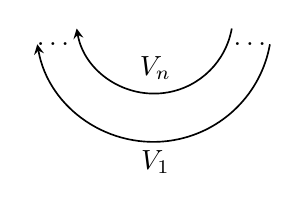
\begin{tikzpicture}[baseline=-1cm]
		\tikzsetup
		\node at (0.2,0) {$\dots$};
		\node at (2.7,0) {$\dots$};
		\draw[tikzdefault,<-] (0,0) arc(190:350:1.5cm);
		\node at(1.5,-1.5) {$V_1$};
		\draw[tikzdefault,<-] (0.5,0.2) arc(190:350:1cm);
		\node at(1.5,-0.3) {$V_n$};
	\end{tikzpicture}
}
%%%%%%%%%%%%%%%%%%%%%%%%%%

%%%%%%%%%%%%%%%%%%%%%%%%%%
\newcommand{\tzPairingV}{
	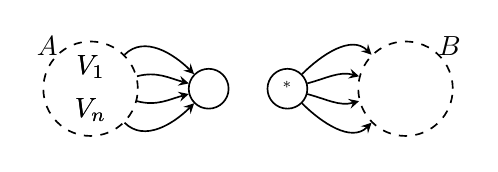
\begin{tikzpicture}[baseline=0pt]
		\tikzsetup
		\node[circle, draw, dashed, minimum size=1.2cm,label=135:$A$] (A) at (0,0)
		{} ;
		\node[morphism] (ph) at (1.5,0) {$\ph$};
		\node[morphism] (ph') at (2.5,0) {$\ph^*$};
		\node[circle, draw, dashed, minimum size=1.2cm, label=45:$B$] (B) at (4,0)
		{};
		\draw[tikzdefault, ->, out=45,in=135] (A) to (ph) 
		node[pos=0.5,above] {$V_1$};
		\draw[tikzdefault, ->,out=15,in=165] (A) to (ph);
		\draw[tikzdefault, ->,out=-15,in=195] (A) to (ph);
		\draw[tikzdefault, ->,out=-45,in=225] (A) to (ph) 
		node[pos=0.5,below] {$V_n$};
		\draw[tikzdefault, ->,out=45,in=135] (ph') to (B) 
		node[pos=0.5,above] {$V_1$};
		\draw[tikzdefault, ->,out=15,in=165] (ph') to (B);
		\draw[tikzdefault, ->,out=-15,in=195] (ph') to (B);
		\draw[tikzdefault, ->,out=-45,in=225] (ph') to (B) 
		node[pos=0.5,below] {$V_n$};
	\end{tikzpicture}
}

%%%%%%%%%%%%%%%%%%%%%%%%%%
\newcommand{\tzPairingVI}{
	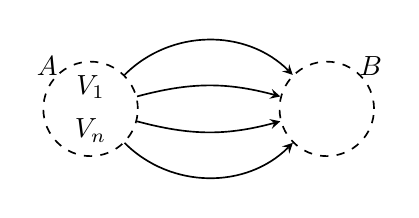
\begin{tikzpicture}[baseline=0pt]
		\tikzsetup
		\node[circle, draw, dashed, minimum size=1.2cm,label=135:$A$] (A) at (0,0)
		{};
		\node[circle, draw, dashed, minimum size=1.2cm,label=45:$B$] (B) at (3,0)
		{};
		\draw[tikzdefault, ->,out=45,in=135] (A) to (B) 
		node[pos=0.5,above] {$V_1$};
		\draw[tikzdefault, ->,out=15,in=165] (A) to (B);
		\draw[tikzdefault, ->,out=-15,in=195] (A) to (B);
		\draw[tikzdefault, ->,out=-45,in=225] (A) to (B) 
		node[pos=0.5,below] {$V_n$};
	\end{tikzpicture}
}
%%%%%%%%%%%%%%%%%%%%%%%%%%

%%%%%%%%%%%%%%%%%%%%%%%%%%%
\newcommand{\tzPairingVII}{
	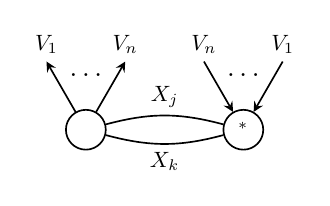
\begin{tikzpicture}[baseline=0pt]
		\tikzsetup
		\node[morphism] (ph) at (0,0) {$\ph$};
		\node[morphism] (ph*) at (2,0) {$\ph^*$};
		\node at (0,0.7) {$\dots$};
		\node at (2,0.7) {$\dots$};
		\draw[tikzdefault,->] (ph)-- +(120:1cm) node[pos=1.0,above,scale=0.8]
		{$V_1$};
		\draw[tikzdefault,->] (ph)-- +(60:1cm) node[pos=1.0,above,scale=0.8]
		{$V_n$};
		\draw[tikzdefault,<-] (ph*)-- +(120:1cm) node[pos=1.0,above,scale=0.8]
		{$V_n$};
		\draw[tikzdefault,<-] (ph*)-- +(60:1cm) node[pos=1.0,above,scale=0.8]
		{$V_1$};
		\draw[tikzdefault,out=15,in=165] (ph) to node[pos=0.5,above,scale=0.8] {$X_j$} (ph*);
		\draw[tikzdefault,out=-15,in=195] (ph) to node[pos=0.5,below,scale=0.8] {$X_k$} (ph*);
	\end{tikzpicture}
}
%%%%%%%%%%%%%%%%%%%%%%%%%%

%%%%%%%%%%%%%%%%%%%%%%%%%%%
\newcommand{\tzPairingVIII}{
	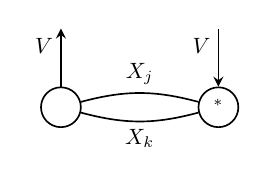
\begin{tikzpicture}[baseline=0pt]
		\tikzsetup
		\node[morphism] (ph) at (0,0) {$\ph$};
		\node[morphism] (ph*) at (2,0) {$\ph^*$};
		\draw[tikzdefault,->] (ph)-- +(90:1cm) node[pos=0.7,left,scale=0.8] {$V$};
		\draw[tikzdefault,<-] (ph*)--  +(90:1cm) node[pos=0.7,left,scale=0.8]
		{$V$};
		\draw[tikzdefault,out=15,in=165] (ph) to node[pos=0.5,above,scale=0.8] {$X_j$} (ph*) ;
		\draw[tikzdefault,out=-15,in=195] (ph) to node[pos=0.5,below,scale=0.8] {$X_k$} (ph*) ;
	\end{tikzpicture}
}
%%%%%%%%%%%%%%%%%%%%%%%%%%

%%%%%%%%%%%%%%%%%%%%%%%%%%%
\newcommand{\tzPairingIX}{
	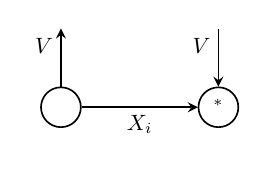
\begin{tikzpicture}[baseline=0pt]
		\tikzsetup
		\node[morphism] (ph) at (0,0) {$\ph$};
		\node[morphism] (ph*) at (2,0) {$\ph^*$};
		\draw[tikzdefault,->] (ph)-- +(90:1cm) node[pos=0.7,left,scale=0.8] {$V$};
		\draw[tikzdefault,<-] (ph*)--  +(90:1cm) node[pos=0.7,left,scale=0.8]
		{$V$};
		\draw[tikzdefault,->] (ph) -- (ph*) node[pos=0.5,below,scale=0.8] {$X_i$};
	\end{tikzpicture}
}
%%%%%%%%%%%%%%%%%%%%%%%%%%

%%%%%%%%%%%%%%%%%%%%%%%%%%%
\newcommand{\tzMoveMtwoI}{
	\begin{tikzpicture}[baseline=0pt]
		\tikzsetup
		\node[morphism] (ph) at (0,0) {$\ph_\al$};
		\node[morphism] (psi) at (2,0) {$\psi_\be$};
		\node at (0,0.7) {$\dots$};
		\node at (2,0.7) {$\dots$};
		\draw[tikzdefault,->] (ph)-- +(120:1cm) node[pos=1.0,above,scale=0.8]
		{$V_1$};
		\draw[tikzdefault,->] (ph)-- +(60:1cm) node[pos=1.0,above,scale=0.8]
		{$V_n$};
		\draw[tikzdefault,<-] (psi)-- +(120:1cm) node[pos=1.0,above,scale=0.8]
		{$W_m$};
		\draw[tikzdefault,<-] (psi)-- +(60:1cm) node[pos=1.0,above,scale=0.8]
		{$W_1$};
		\draw[tikzdefault,->] (ph) -- (psi) node[pos=0.5,below,scale=0.8] {$X_i$}; 
	\end{tikzpicture}
}
%%%%%%%%%%%%%%%%%%%%%%%%%%

%%%%%%%%%%%%%%%%%%%%%%%%%%%
\newcommand{\tzMoveMtwoII}{
	\begin{tikzpicture}[baseline=0pt]
		\tikzsetup
		\node[morphism] (ph) at (2,0) {$\ph^\al$};
		\node[morphism] (psi) at (0,0) {$\psi^\be$};
		\node at (0,0.7) {$\dots$};
		\node at (2,0.7) {$\dots$};
		\draw[tikzdefault,<-] (ph)-- +(120:1cm) node[pos=1.0,above,scale=0.8]
		{$V_n$};
		\draw[tikzdefault,<-] (ph)-- +(60:1cm) node[pos=1.0,above,scale=0.8]
		{$V_1$};
		\draw[tikzdefault,->] (psi)-- +(120:1cm) node[pos=1.0,above,scale=0.8]
		{$W_1$};
		\draw[tikzdefault,->] (psi)-- +(60:1cm) node[pos=1.0,above,scale=0.8]
		{$W_m$};
		\draw[tikzdefault,->] (psi) -- (ph) node[pos=0.5,below,scale=0.8] {$X^*_i$}; 
	\end{tikzpicture}
}
%%%%%%%%%%%%%%%%%%%%%%%%%%

%%%%%%%%%%%%%%%%%%%%%%%%%%%
\newcommand{\tzMoveMtwoIII}{
	\begin{tikzpicture}[baseline=0pt]
		\tikzsetup
		\node[coupon] (ph) at (0,0) {$\ph_\al\ccc{X_i}\psi_\be$};
		\draw[tikzdefault,->] (ph.150)-- +(110:1cm) node[pos=1.0,above left,scale=0.8]
		{$V_1$};
		\draw[tikzdefault,->] (ph.130)-- +(110:1cm) node[pos=1.0,above,scale=0.8]
		{$V_n$};
		\draw[tikzdefault,<-] (ph.50)-- +(70:1cm) node[pos=1.0,above,scale=0.8]
		{$W_m$};
		\draw[tikzdefault,<-] (ph.30)-- +(70:1cm) node[pos=1.0,above right,scale=0.8]
		{$W_1$};
	\end{tikzpicture}
}
%%%%%%%%%%%%%%%%%%%%%%%%%%

%%%%%%%%%%%%%%%%%%%%%%%%%%%
\newcommand{\tzMoveMtwoIV}{
	\begin{tikzpicture}[baseline=0pt]
		\tikzsetup
		\node[coupon] (ph) at (0,0) {$\psi^\be\ccc{X_i}\ph^\al$};
		\draw[tikzdefault,<-] (ph.150)-- +(110:1cm) node[pos=1.0,above left,scale=0.8]
		{$W_1$};
		\draw[tikzdefault,<-] (ph.130)-- +(110:1cm) node[pos=1.0,above,scale=0.8]
		{$W_m$};
		\draw[tikzdefault,->] (ph.50)-- +(70:1cm) node[pos=1.0,above,scale=0.8]
		{$V_m$};
		\draw[tikzdefault,->] (ph.30)-- +(70:1cm) node[pos=1.0,above right,scale=0.8]
		{$V_n$};
	\end{tikzpicture}
}
%%%%%%%%%%%%%%%%%%%%%%%%%%%
